\subsection{Serviço de Backups}

O servidor de \emph{Backups} utilizado neste caso é o Servidor \emph{Arkeia}.

O \emph{Arkeia} é uma excelente solução para a salvaguarda de dados sendo um auxiliar importante em acções de \emph{disaster recovery}. O \emph{Arkeia} oferece uma resposta cabal em termos de desempenho, flexibilidade e confiabilidade para todo o tipo e volume dados a salvaguardar.

O \emph{Arkeia} é rápido, fácil de usar, sendo compatível com praticamente qualquer combinação de computadores, sistemas operativos e dispositivos de armazenamento. A salvaguarda de dados pode facilmente ser feita de forma global ou incremental preservando a estrutura de directorias, \emph{links} simbólicos e quaisquer atributos especiais do sistema de ficheiros.

Para determinadas plataformas existe a possibilidade de aquisição de \textit{plugins} para efectuar \textit{Hot Backups} de dados do Oracle, MySQL, etc.

Informações adicionais podem ser obtidas em:\\ \begin{normalsize}\sffamily\href{http://www.arkeia.com/products/arkeianetworkbackup/index.php}{www.arkeia.com/products/arkeianetworkbackup/index.php}\end{normalsize}

As várias configurações do \emph{Arkeia} podem ser encontradas na seguinte directoria:

\begin{Verbatim}[commandchars=\\\{\}]
/opt/arkeia/arkeiad
\end{Verbatim}

O comando para controlar este serviço (iniciar/parar) é o seguinte:

\begin{Verbatim}[commandchars=\\\{\}]
# /etc/rc.d/init.d/arkeia start
# /etc/rc.d/init.d/arkeia stop
\end{Verbatim}

Caso o cliente tenha adquirido a opção de Disaster Recovery a mesma permite-lhe efectuar a recuperação de todo o sistema operativo aquando da criação do backup. Deste modo o cliente está seguro em caso de falha de hardware como um disco avariado.

Informações adicionais podem ser obtidas em:\\ \begin{normalsize}\sffamily\href{http://www.arkeia.com/products/arkeiaoptions/disaster\_recovery.php}{www.arkeia.com/products/arkeiaoptions/disaster\_recovery.php}\end{normalsize}

As máquinas às quais se desejam fazer \textit{backups} deverão ter instalado o cliente Arkeia. Este está disponível para vários sistemas operativos, podendo ser descarregado no seguinte endereço: \url{ftp://ftp.arkeia.com/arkeia-software-application/arkeia-10.0/arkeia-network-backup/}

O acesso à interface deverá ser feito através da URL http://XXX.XXX.XXX.XXX:20617/ onde XXX.XXX.XXX.XXX é o endereço ip do seu servidor de backup.

\begin{figure}[H]
    \begin{center}
        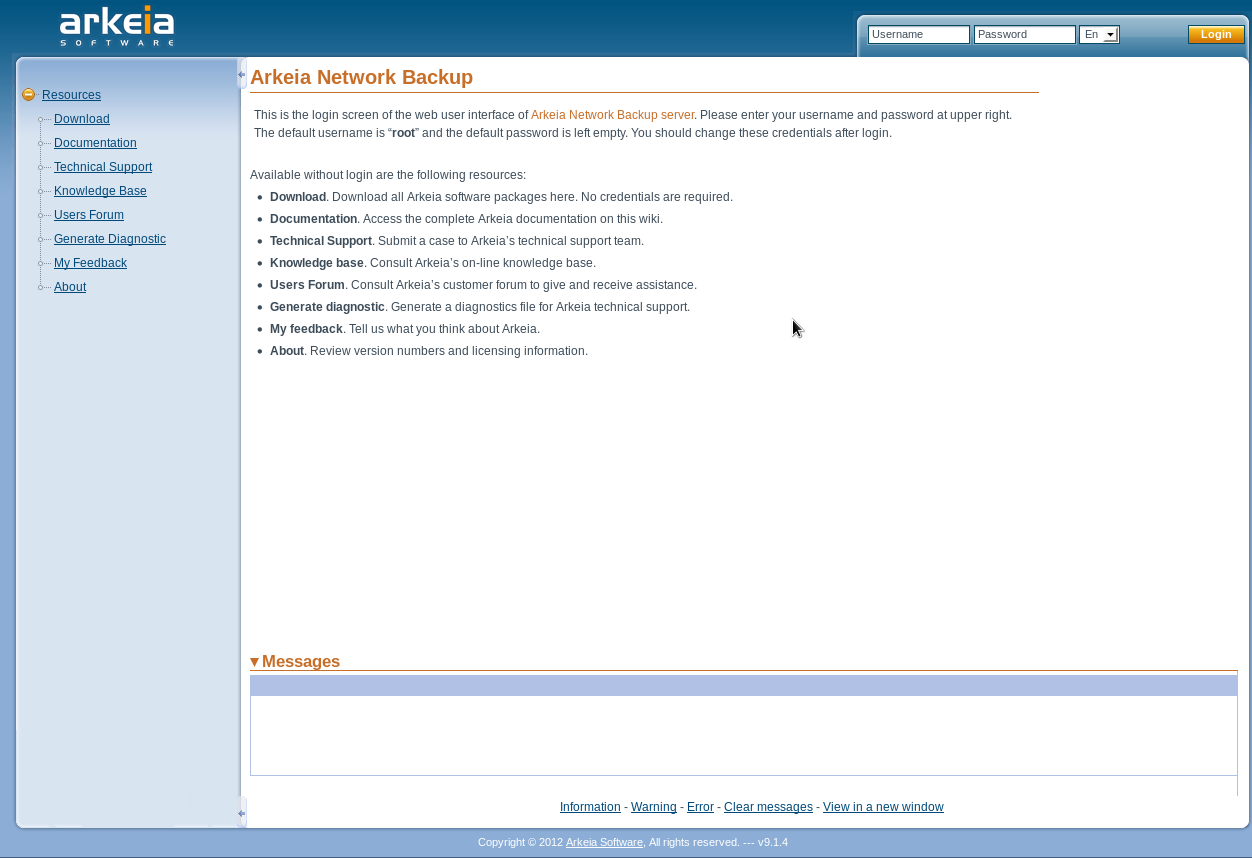
\includegraphics[width=15cm]{include/img/arkeia1.png}
    \end{center}
    \caption{Interface de login do Arkeia}
    \label{fig:arkeia1}
\end{figure}

Após o login, em "configure" -> "clients", deverá ser possível obter uma lista dos clientes que já têm o agente instalado e correctamente configurado, cf. figura \ref{fig:arkeia2}

\begin{figure}[H]
    \begin{center}
        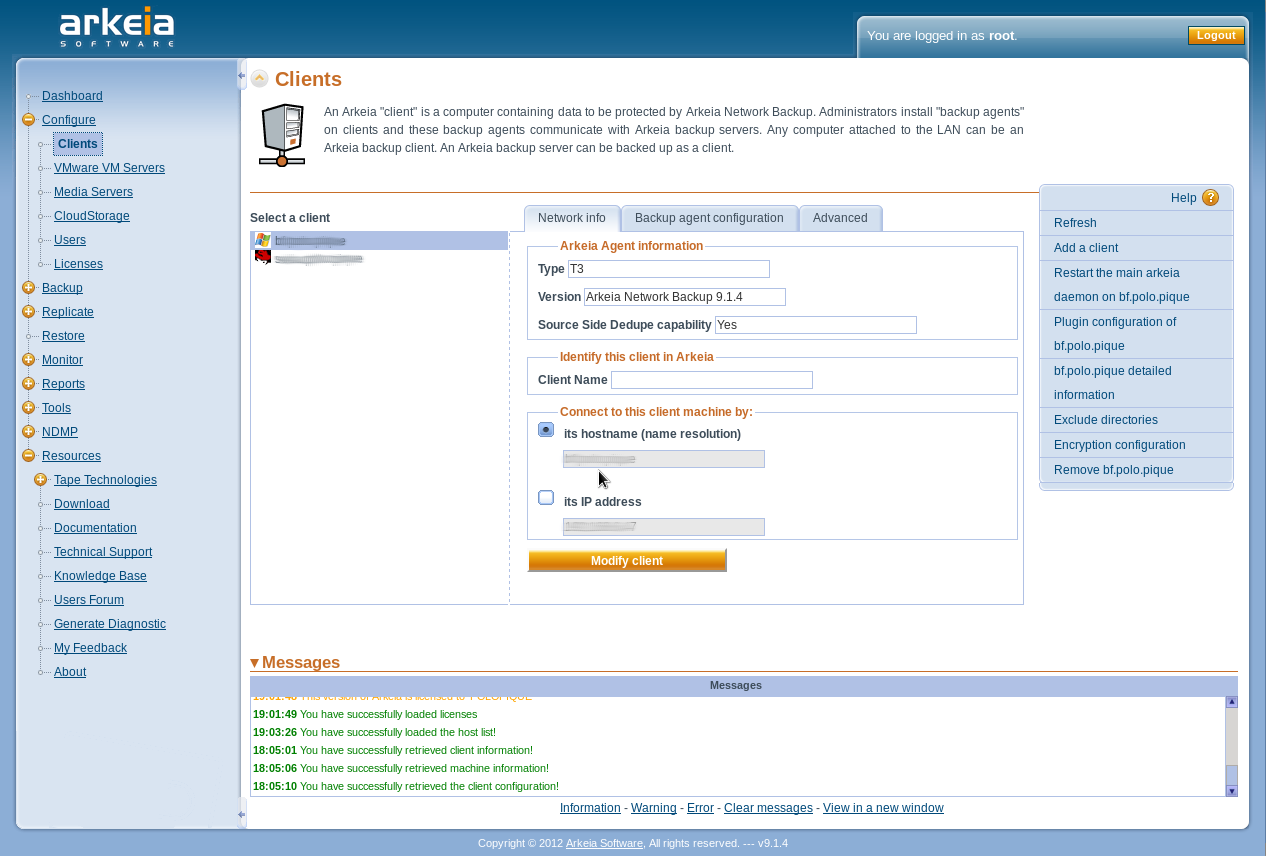
\includegraphics[width=15cm]{include/img/arkeia2.png}
    \end{center}
    \caption{Clientes Arkeia}
    \label{fig:arkeia2}
\end{figure}
